\documentclass[aspectratio=169]{beamer}

\usepackage{ccicons}
\usepackage{fontspec}
\usepackage{import}
\usepackage{listings}
\usepackage{tikz}

\subimport{../}{colors.tex}

\usetikzlibrary{
  arrows,
  arrows.meta,
  automata,
  backgrounds,
  calc,
  chains,
  decorations.pathreplacing,
  fit,
  matrix,
  overlay-beamer-styles,
  positioning,
  shapes,
  tikzmark,
}
\usetikzmarklibrary{listings}

\hypersetup{
  colorlinks=true,
  urlcolor=uclablue,
}

\setbeamercolor{frametitle}{fg=primarycolor}
\setbeamercolor{structure}{fg=primarycolor}
\setbeamercolor{enumerate item}{fg=black}
\setbeamercolor{itemize item}{fg=black}
\setbeamercolor{itemize subitem}{fg=black}

\setbeamersize{text margin left=26.6mm}
\addtolength{\headsep}{2mm}

\setbeamertemplate{navigation symbols}{}
\setbeamertemplate{headline}{}
\setbeamertemplate{footline}{}
\setbeamertemplate{itemize item}{\color{black}}
\setbeamertemplate{itemize items}[circle]

\setbeamertemplate{footline}{
  \begin{tikzpicture}[remember picture,
                      overlay,
                      shift={(current page.south west)}]
    \node [black!50, inner sep=2mm, anchor=south east]
          at (current page.south east) {\footnotesize \insertframenumber};
  \end{tikzpicture}
}

\setsansfont{Overpass}[Scale=MatchLowercase]
\setmonofont{Overpass Mono}[Scale=MatchLowercase]

\makeatletter
\newcommand\version[1]{\renewcommand\@version{#1}}
\newcommand\@version{}
\def\insertversion{\@version}

\newcommand\lecturenumber[1]{\renewcommand\@lecturenumber{#1}}
\newcommand\@lecturenumber{}
\def\insertlecturenumber{\@lecturenumber}
\makeatother

\setbeamertemplate{title page}
{
  \begin{tikzpicture}[remember picture,
                      overlay,
                      shift={(current page.south west)},
                      background rectangle/.style={fill=uclablue},
                      show background rectangle]
    \node [anchor=west, align=left, inner sep=0, text=white]
          (lecturenumber) at (\paperwidth / 6, \paperheight * 3 / 4)
          {\Large Lecture \insertlecturenumber};
    \node [inner sep=0, align=left, text=white, node distance=0,
           above left=of lecturenumber, anchor=south west, yshift=2mm]
          {\Large CS 111: Operating System Principles};
    \node (title) [inner sep=0, anchor=west, align=right, text=white]
          at (\paperwidth / 6, \paperheight / 2)
          {{\bfseries \Huge \inserttitle{}}};
    \node [inner sep=0, align=right, text=white, node distance=0,
           below right=of title, anchor=north east, yshift=-1mm]
          {{\footnotesize \ttfamily \insertversion}};
    \node [inner sep=0, text=white, align=left, anchor=west]
          (author) at (\paperwidth / 6, \paperheight / 4)
          {\insertauthor};
    \node [text=white, inner sep=0, align=left, node distance=0,
           below left=of author, anchor=north west, yshift=-2mm]
          {\insertdate};
    \node [align=right, anchor=south east, inner sep=2mm, text=white]
          (license) at (\paperwidth, 0)
          {\footnotesize This  work is licensed under a
           \href{http://creativecommons.org/licenses/by-sa/4.0/}
                {\color{uclagold} Creative Commons Attribution-ShareAlike 4.0
                 International License}};
    \node [text=white, inner sep=0, align=right, node distance=0,
           above right=of license, anchor=south east, xshift=-2mm]
          {\Large \ccbysa};
  \end{tikzpicture}
}

\tikzset{
  >=Straight Barb[],
  shorten >=1pt,
  initial text=,
}

\lstset{
  basicstyle=\footnotesize\ttfamily,
}


\lecturenumber{21}
\title{Virtual Machines}
\version{1.0.0}
\author{Jon Eyolfson}
\date{May 27, 2021}

\begin{document}
  \begin{frame}[plain, noframenumbering]
    \titlepage
  \end{frame}

  \begin{frame}{Virtual Machines Abstract an Entire Machine}

    Goal: run multiple operating systems on a single machine

    \hspace{2em} Each OS believes they're the only one running

    \vspace{2em}

    We used it for our Labs to make sure we all had the same environment

    \hspace{2em} It was a full Linux install with all the software you needed
  \end{frame}

  \begin{frame}{The Host Has Direct Control Over the Hardware}

    The \textit{hypervisor} or \textit{virtual machine manager} (VMM) controls
    virtual machines

    \hspace{2em} Creation, management, isolation (which hardware is it able to
    access)

    \vspace{2em}

    There are two kinds of hypervisors: type 1 and type 2

    \hspace{2em} Type 1: bare metal hypervisor, it runs directly on the host's
    hardware

    \hspace{4em} Requires special hardware support

    \hspace{2em} Type 2: hosted hypervisor, it simulates a hypervisor and runs
                 as an application

    \hspace{4em} Slower, but does not require any special hardware

    \vspace{2em}

    A \textit{guest} sees it's own virtual copy of the host
  \end{frame}

  \begin{frame}{(a) Is a Typical Machine (b) Shows One Machine Running 3 Kernels}
    \begin{center}
      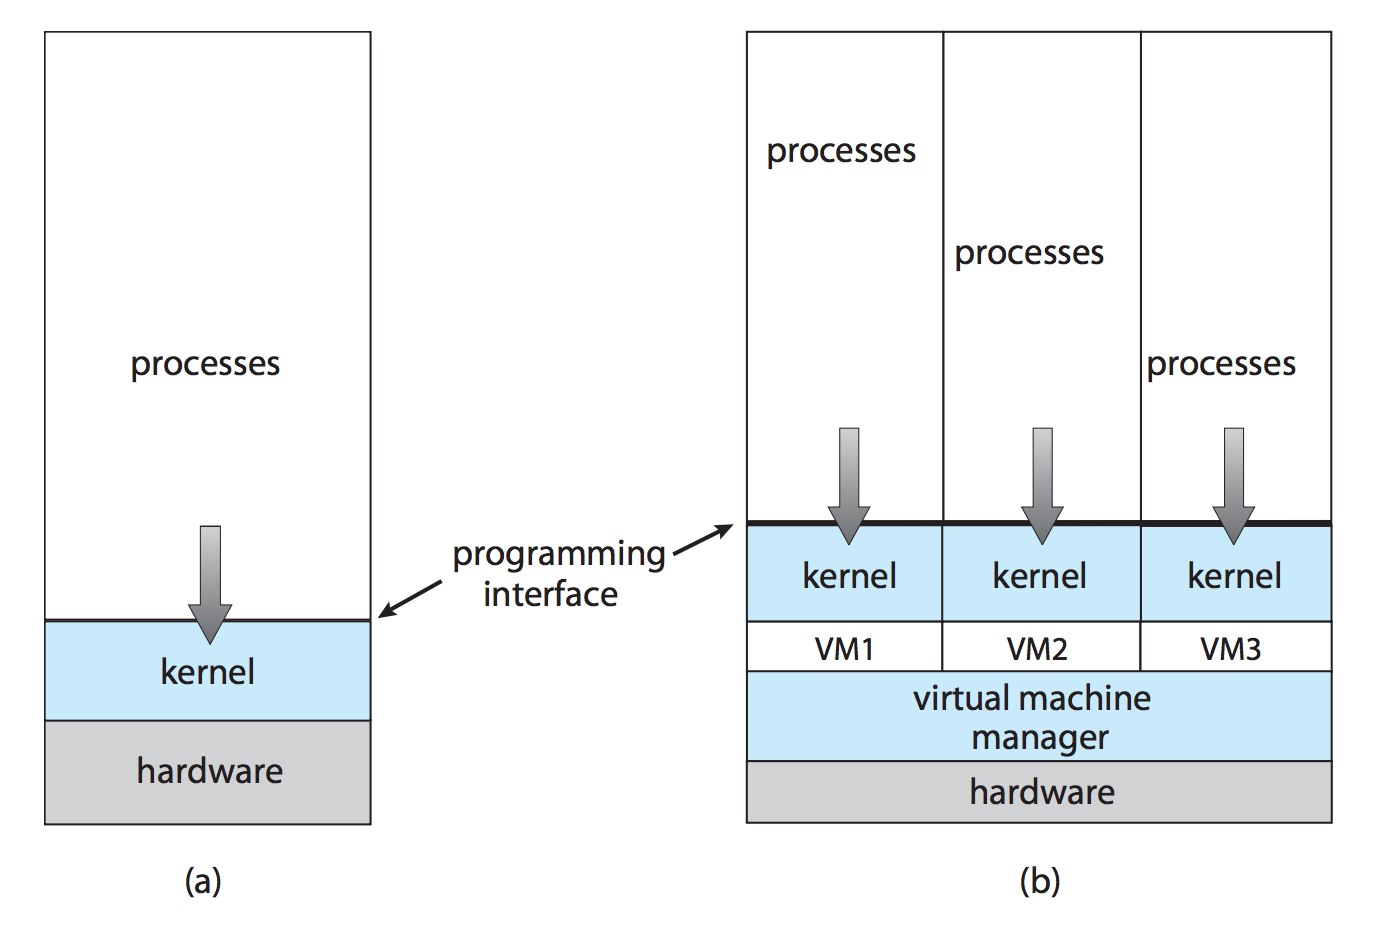
\includegraphics[width=0.8\textwidth]{non-virtual-machine.png}
    \end{center}
  \end{frame}

  \begin{frame}
    \frametitle{Virtual Machines are Not Emulation}

    Emulation is typically used to translate one ISA to another

    \hspace{2em} e.g. x86\_64 to ARM/RISC-V

    \vspace{2em}

    Our guest operating system executes instructions directly using the same ISA

    \hspace{2em} Otherwise translating instructions is typically slow

    \vspace{2em}

    It's OK for some uses, such as a Nintendo Entertainment System (NES)
    emulator

    \vspace{2em}

    A virtual machine could use emulation to run a virtual machine for a
    different ISA

    \hspace{2em} Performance would suffer greatly
  \end{frame}

  \begin{frame}
    \frametitle{Virtual Machines Enable Pause and Play}

    Much like our kernel can pause a process, a hypervisor can pause an OS

    \vspace{2em}

    The hypervisor needs to context switch between  virtual machines

    \hspace{2em} It'll save the current state and restores it later

    \vspace{2em}

    We could also move it around, exactly like a process
  \end{frame}

  \begin{frame}
    \frametitle{Virtual Machines Provide Protection Through Isolation}

    The guests are isolated from each other, and the host

    \vspace{2em}

    The hypervisor and set limits on: CPU time, memory, network bandwidth, etc.

    \hspace{2em} A compromised guest only has access to it's own virtualized
                 hardware

    \vspace{2em}

    You can easily roll back the infected virtual machine, or remove it
  \end{frame}

  \begin{frame}{Virtual Machines Also Help Consolidation}

    In data centers there's many servers running, often not making use of all
    resources

    \hspace{2em} Servers with different purposes could be sharing the same
                 hardware

    \vspace{2em}

    Instead of having lightly used physical systems, make them virtual machines

    \hspace{2em} Run as many on a single machine as possible
  \end{frame}

  \begin{frame}
    \frametitle{A Virtual CPU (VCPU) Is the Key Abstraction}

    For processes, part of the process control block (PCB) acted as a virtual
    CPU

    \hspace{2em} It doesn't virtualize all parts of the CPU, just enough for
                 user-mode processes

    \vspace{2em}

    The VCPU is a data structure that stores the state of the CPU

    \hspace{2em} The hypervisor saves this when the guest isn't running

    \vspace{2em}

    When the virtual machine resumes, like the PCB, it loads the data and
    resumes
  \end{frame}

  \begin{frame}{The Guest Still Uses User and Kernel Modes}

    There are no changes to the guest operating systems

    \hspace{2em} A Linux kernel still uses privileged instructions

    \vspace{2em}

    Recall on x86\_64 user mode is ring 3, kernel mode is ring 0

    \hspace{2em} A hardware hypervisor (type 1) is ring -1, letting it control the guest

    \vspace{2em}

    For type 2 hypervisors, the host has to create a virtual kernel and user mode
  \end{frame}

  \begin{frame}
    \frametitle{One Strategy is to Trap-and-Emulate}

    For type 2 hypervisors the guest runs on the host in user mode

    \hspace{2em} Any privileged instructions generate a trap (wrong mode)

    \vspace{2em}

    The hypervisor should explicitly handle this error

    \hspace{2em} Emulate (or simulate) the operation for the guest and resume it

    \vspace{2em}

    This will slow down the otherwise native execution
  \end{frame}

  \begin{frame}{Trap-and-Emulate Visually}
    \begin{center}
      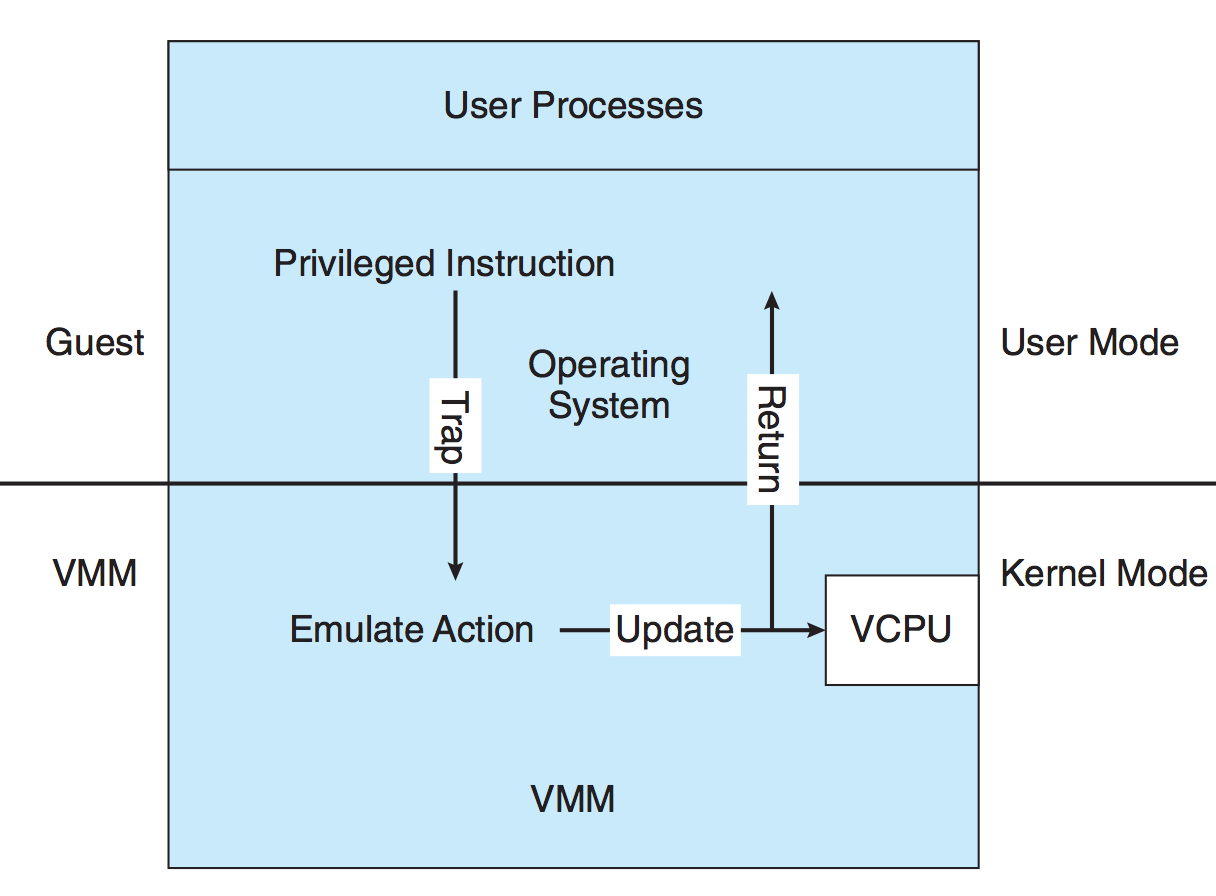
\includegraphics[width=0.75\textwidth]{trap-and-emulate.png}
    \end{center}
  \end{frame}

  \begin{frame}{Trap-and-Emulate Does Not Always Work}

     Some CPUs are not clear between privileged and non-privileged instructions

     \hspace{2em} This includes x86\_64, virtual machines didn't exist in the 1970s

     \vspace{2em}

     One example is the \texttt{popf} instruction, it loads the flags register
     from the stack

     \hspace{2em} It behaves differently for both kernel and user mode

     \vspace{2em}

     It does not generate a trap, so you can't trap-and-emulate

     \hspace{2em} These \textit{special} instructions need another approach
  \end{frame}

  \begin{frame}{Special Instructions Need Binary Translation}

    If the guest VCPU is in user mode, we can run instructions natively

    \hspace{2em} in kernel mode, the hypervisor inspects every instruction
                 before execution

    \vspace{2em}

    Special instructions need to be translated to instructions with the same
    effect

    \hspace{2em} Regular instructions can run natively

    \vspace{2em}

    The kernel uses a CPU instruction to switch from user to kernel mode

    \hspace{2em} The hypervisor can handle that using normal trap-and-emulate

    \vspace{2em}

    Overall performance for type 2 hypervisors suffer, but they're adequate
  \end{frame}

  \begin{frame}{Binary Translation Visually}
    \begin{center}
      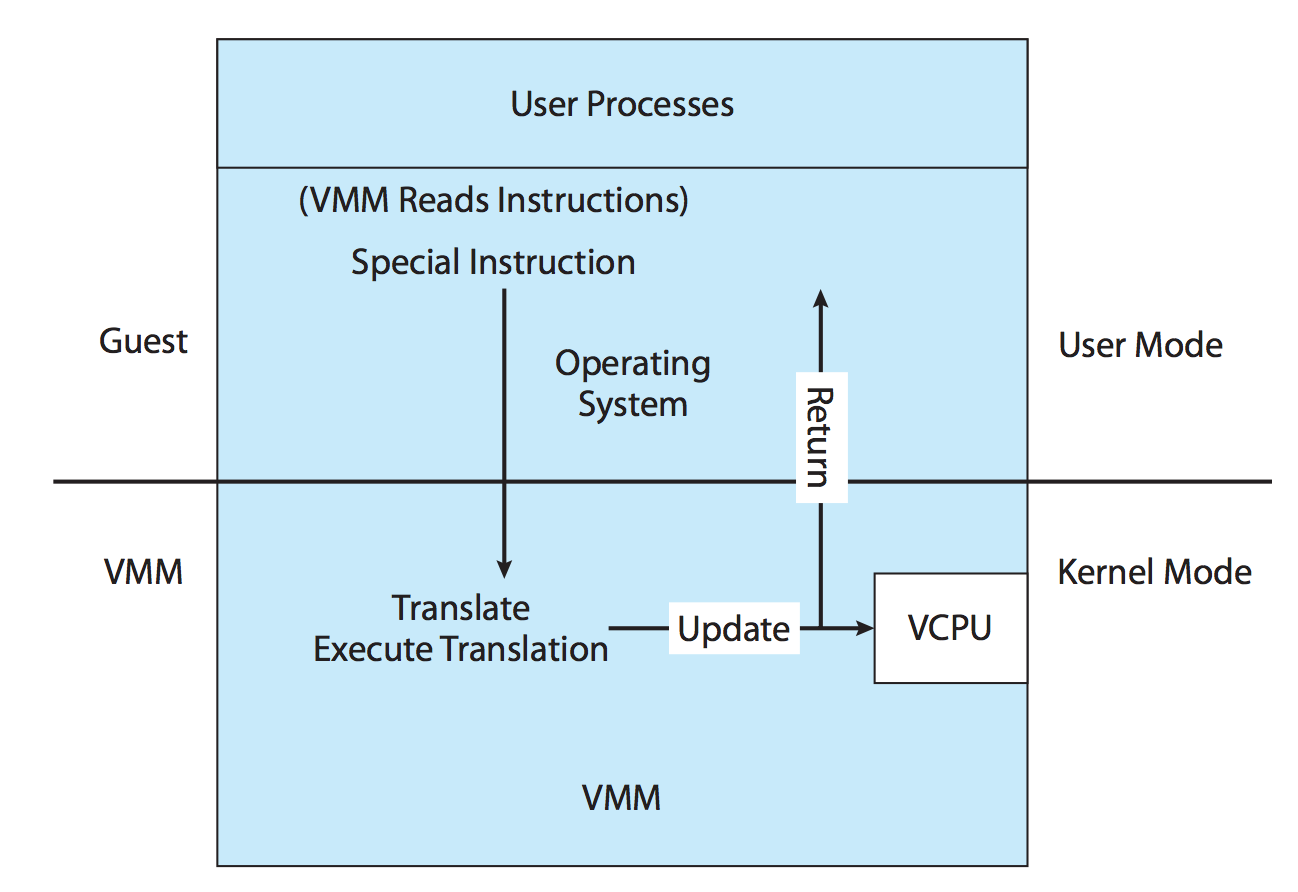
\includegraphics[width=0.75\textwidth]{binary-translation.png}
    \end{center}
  \end{frame}

  \begin{frame}{One More Hardware Rescue}

    In 2005 Intel introduced virtualization as VT-x and in 2006 AMD did as AMD-V

    \hspace{2em} Intel's codename Vanderpool, published as Virtual
                 Machine Extensions (VMX)

    \hspace{2em} AMD's codename Pacifica, published as Secure Virtual
                 Machine (SVM)

    \vspace{2em}

    This added the concept of ring -1, or hypervisor mode

    \vspace{2em}

    The host kernel claims the hypervisor, and is the only one able to access
    it

    \hspace{2em} It can set the isolation for the guests and what hardware
                 to virtualize
  \end{frame}

  \begin{frame}{Virtualized Scheduling}

    If there is only one CPU on the physical machine, the guest will not know

    \hspace{2em} The host could still present multiple virtual CPUs to the guest

    \vspace{2em}

    We now need to map the VCPUs to physical CPUs, or schedule them like
    processes

    \hspace{2em} Like a normal kernel, there will also be hypervisor threads
  \end{frame}

  \begin{frame}{One Approach is CPU Assignment}

    If there are more physical cores on the host than all VCPUs, we can map 1:1

    \hspace{2em} The host can continue using the spare physical cores

    \vspace{2em}

    If we have to share, things get more complicated (called overcommitting)

    \hspace{2em} At equal numbers we can still map 1:1, the hypervisor threads
                 don't run often

    \vspace{2em}

    We have to use a scheduling algorithm, like we used for processes
  \end{frame}

  \begin{frame}{CPU Overcommitment Causes Additional Problems}

    The guest operating system runs too unpredictably for soft real-time tasks

    \hspace{2em} It may be context switched out when the user process says not
    to

    \vspace{2em}

    For example, consider a real-time round robin time slice is 10~ms

    \hspace{2em} The guest will not have a consistent slice of 10~ms, it may be
                 much higher

    \vspace{2em}

    This may make processes miss deadlines they wouldn't have running on the host

    \hspace{2em} In this case virtualization has different observable behavior
  \end{frame}

  \begin{frame}{Virtualized Memory Management Gets a Lot More Complex}

    Recall: virtual memory allows each process to think it has the entire
            address space

    \vspace{2em}

    Now the guest kernel thinks it's managing the entire physical address space

    \hspace{2em} We have to virtualize that too!

    \vspace{2em}

    The problem gets even worse if memory is overcommitted as well
  \end{frame}

  \begin{frame}{Nested Page Tables Enable Virtual Memory for Guest Kernels}

    The guest thinks it controls physical memory, and does page table management

    \vspace{2em}

    The hypervisor maintains a nested page table the re-translates for the guest

    \hspace{2em} It translates the guest's page able to the real physical page
                 table

    \vspace{2em}

    For overcommitted memory the hypervisor can provide double-paging

    \hspace{2em} The hypervisor does its own page replacement algorithm

    \hspace{4em} However, the guest may know it's memory access patterns better
  \end{frame}

  \begin{frame}{Guests Could Share Pages if They're Duplicates}

    Similar to copy-on-write pages, we can get memory saves by sharing pages

    \hspace{2em} This time instead of sharing between processes, share between
                 guests

    \vspace{2em}

    The hypervisor can do duplicate detection by hashing the contents of pages

    \hspace{2em} If two hashes are the same, check they're the same
                 byte-for-byte

    \vspace{2em}

    If they're the same, we can share them until one of the guests try to write

    \hspace{2em} Then we again do copy-on-write as before
  \end{frame}

  \begin{frame}{The Hypervisor Provides Virtualized I/O Devices}

    The hypervisor can multiplex one device to multiple virtual machines

    \hspace{2em} The hypervisor could also emulate devices that don't
                 physically exist

    \vspace{2em}

    The hypervisor could also map one physical device to a virtual device
    one VM

    \hspace{2em} The VM has exclusive access to the device, but hypervisor
                 still translates

    \vspace{2em}

    There is a hardware solution to remove the hypervisor during run-time ---
    IOMMU

    \hspace{2em} The hypervisor maps the devices virtual memory exclusively
                 to the guest

    \hspace{4em} The VM now actually has exclusive control over the device

    \hspace{6em} This allows complex GPUs to work at native speeds in VMs
  \end{frame}

  \begin{frame}{Virtual Machines Boot from a Virtualized Disk}

    You create a \textit{disk image} that has all the contents of a physical
    disk

    \hspace{2em} It contains partitions, and each partition has a file system

    \vspace{2em}

    Usually, it's one big file (but some formats allow you to split it up)

    \hspace{2em} The guest kernel sees it has a normal disk, that it has full
                 control of

    \vspace{2em}

    The disk image is all you need for the virtual machine, makes it easy to
    move

    \hspace{2em} The \texttt{ova} file you downloaded is basically a disk image
                 and guest settings
  \end{frame}

  \begin{frame}{Virtual Machines Enable Live Migration}

    You can migrate a virtual machine from one physical machine to another

    \vspace{2em}

    Users using the guest can't tell that the guest moved physical machines

    \hspace{2em} Usually, it's a long process: you have to tell the users

    \vspace{2em}

    This is how cloud providers try to balance the load

    \hspace{2em} They move VMs off of overloaded machines
  \end{frame}

  \begin{frame}{Live Migration in 8 Easy Steps}
    \begin{enumerate}
      \item The source hypervisor connects to the destination hypervisor.
      \item The destination creates a configuration for a new guest
      \item The source sends all read-only memory pages to the destination
      \item The source sends all read-write pages (marking them as clean)
      \item Any pages that were modified during the previous step (if any)

            are sent and marked as clean. 
      \item If there were few pages that were dirty in the previous two steps,

             the source freezes the guest, sends the final state and any final
             dirty pages
      \item The destination acknowledges receipt and begins execution of the guest
      \item The source terminates the guest
    \end{enumerate}
  \end{frame}

  \begin{frame}{Live Migration Visually}
    \begin{center}
      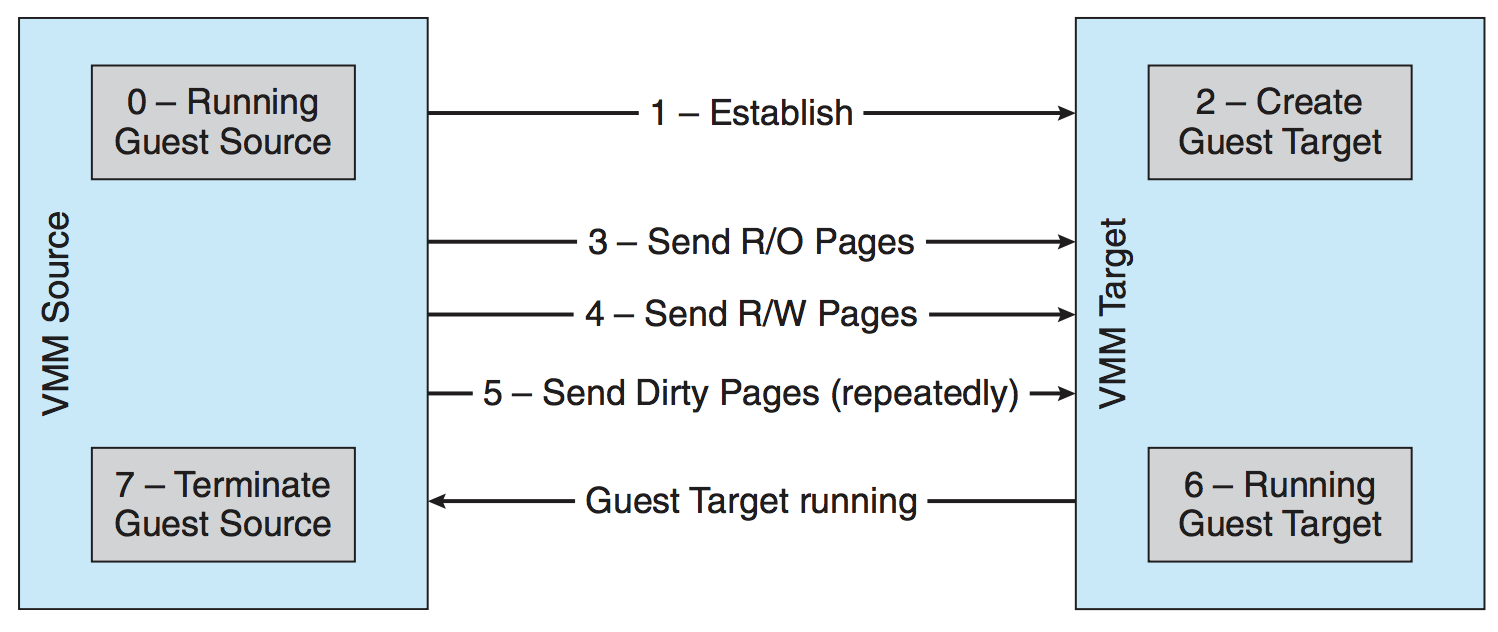
\includegraphics[width=0.9\textwidth]{live-migration.png}
    \end{center}
  \end{frame}

  \begin{frame}{Virtual Machines Could Be Used to Isolate an Application}

    Assume your application uses a dynamic library (back to Lecture 3)

    \hspace{2em} An ABI change would cause your application to no longer work

    \hspace{4em} Even more subtle, the library's behavior could change

    \vspace{2em}

    You may want to freeze your dependencies to deploy it in production

    \hspace{2em} Create a virtual machine for it with all the libraries it
                 needs
  \end{frame}

  \begin{frame}{Containers, like Docker, Aim to be Faster}

    The hypervisor sets limits on: CPU time, memory, network bandwidth, etc.

    \hspace{2em} What if the kernel supported this directly, without
                 virtualization?

    \vspace{2em}

    Linux control groups (\texttt{cgroups}) support hypervisor-like
    limits for processes

    \hspace{2em} Isolate a process to a \textit{namespace}

    \vspace{2em}

    You can set other resources a namespace can access (mount points, IPC, etc.)

    \vspace{2em}

    Containers are lighter-weight than full virtual machines, they use a normal
    kernel
  \end{frame}

  \begin{frame}{Virtual Machines Virtualize a Physical Machine}

    They allow multiple operating systems to share the same hardware
    \begin{itemize}
      \item Virtual machines provide isolation, the hypervisor allocates
            resources
      \item Type 2 hypervisors are slower due to trap-and-emulate and binary
            translation
      \item Type 1 hypervisors are supported by hardware, IOMMU speeds up devices
      \item Hypervisors may overcommit resources and need to physically move VM
      \item Containers aim to have the benefits of VMs, without the overhead
    \end{itemize}
  \end{frame}
\end{document}
